\documentclass{report}
\usepackage{amsmath}
\usepackage{geometry}
\usepackage{graphicx}
\begin{document} 

\begin{flushleft}

\begin{Large}

\textbf{Name - Ankush Vijay Israney} \\
\textbf{Student ID - 14057308} \\
\textbf{CS 613 - Assignment 2 report} \\ 

\end{Large}

\break

\underline { \textbf{PART-1 [Theory Part]}}  \linebreak[2]

Data, M = 
\[
\begin{bmatrix}
-2 & 1 \\
-5 &-4 \\
-3 & 1 \\
0 & 3 \\
-8 & 11 \\
-2 & 5 \\
1 & 0 \\
5 & -1 \\
-1 & -3 \\
6 & 1 \\
\end{bmatrix}
\] \linebreak[2]

X = 
\[
\begin{bmatrix}
-2  \\
-5  \\
-3 \\
0 \\
-8  \\
-2 \\
1  \\
5  \\
-1 \\
6  \\
\end{bmatrix}
\]

Y = 
\[
\begin{bmatrix}
1 \\
-4 \\
1 \\
3 \\
11 \\
5 \\
0 \\
-1 \\
-3 \\
1 \\
\end{bmatrix}
\] \linebreak[2]

Mean, 
\begin{equation}
\mu = -0.9
\end{equation}

Standard Deviation,
\begin{equation}
\sigma = 4.2282
\end{equation}

X - Standardized =
\[
\begin{bmatrix}
-0.2602 \\
-0.9697 \\
-0.4967 \\
0.2129 \\
-1.6792 \\
-0.2602 \\
0.44937 \\
1.3954 \\
-0.0237 \\
1.6319 \\
\end{bmatrix}
\] \linebreak[2]

Adding Bias Feature to X = 
\[
\begin{bmatrix}
1 & -0.2602 \\
1& -0.9697 \\
1 & -0.4967 \\
1 & 0.2129 \\
1 & -1.6792 \\
1 & -0.2602 \\
1 & 0.44937 \\
1 & 1.3954 \\
1 & -0.0237 \\
1 & 1.6319 \\
\end{bmatrix}
\] \linebreak[2]

X\textsuperscript{T} * X = 
\[\begin{bmatrix}
1 & 
1 & 
1 & 
1 & 
1 & 
1 & 
1 & 
1 & 
1 & 
1 \\
-0.2602 &
-0.9697 &
-0.4967 &
0.2129 &
-1.6792 &
-0.2602 &
0.44937 &
1.3954 &
-0.0237 &
1.6319 \\
\end{bmatrix}
\times
\begin{bmatrix}
1 & -0.2602 \\
1 & -0.9697 \\
1 & -0.4967 \\
1 & 0.2129 \\
1 & -1.6792 \\
1 & -0.2602 \\
1 & 0.44937 \\
1 & 1.3954 \\
1 & -0.0237 \\
1 & 1.6319 \\
\end{bmatrix}
\] 


\[=
\begin{bmatrix}
10	& 6.6613e-16 \\
6.6613e-16 & 9 \\
\end{bmatrix}
\] \linebreak[2]

(X\textsuperscript{T} * X)\textsuperscript{-1} =
 \[
\begin{bmatrix}
0.10 & -7.4015e-18 \\
-7.4015e-18 & 0.11 \\
\end{bmatrix}
\]

(X\textsuperscript{T} * X)\textsuperscript{-1} * X\textsuperscript{T} =
 \[
\begin{bmatrix}
0.10 & 0 \\
0 & 0.11 \\
\end{bmatrix}
\times
\begin{bmatrix}
1 & 
1 & 
1 & 
1 & 
1 & 
1 & 
1 & 
1 & 
1 & 
1 \\
-0.2602 &
-0.9697 &
-0.4967 &
0.2129 &
-1.6792 &
-0.2602 &
0.44937 &
1.3954 &
-0.0237 &
1.6319 \\
\end{bmatrix}
\]

\[=
\begin{bmatrix}
0.1 & 0.1 & 0.1 & 0.1 & 0.1 & 0.1 & 0.1 & 0.1 & 0.1 & 0.1 \\
-0.0289 & -0.1077 & -0.0552 & 0.0237 & -0.1866 & -0.0289 & 0.0499 & 0.1550 & -0.0026 &	0.1813
\end{bmatrix}
\] \linebreak[2]

\begin{equation}
Parameters, \theta = ((X\textsuperscript{T} * X)\textsuperscript{-1} * X\textsuperscript{T}) * Y
\end{equation}

\[=
\begin{bmatrix}
0.1 & 0.1 & 0.1 & 0.1 & 0.1 & 0.1 & 0.1 & 0.1 & 0.1 & 0.1 \\
-0.0289 & -0.1077 & -0.0552 & 0.0237 & -0.1866 & -0.0289 & 0.0499 & 0.1550 & -0.0026 &	0.1813
\end{bmatrix}
\times
\begin{bmatrix}
1 \\
-4 \\
1 \\
3 \\
11 \\
5 \\
0 \\
-1 \\
-3 \\
1 \\
\end{bmatrix}
\]

\[=
\begin{bmatrix}
1.400000\\
-1.74489
\end{bmatrix}
\]

\textbf{Final Model:} \linebreak[2]
\begin{equation}
\hat{Y} = \theta_0 + \theta_{1} x_{:, 1}
\end{equation}

\begin{equation}
\hat{Y} = 1.4 + -1.74489*x_{:, 1}
\end{equation}

\break

\underline { \textbf{PART-2 [Simple Closed Form Linear Regression]}}  \linebreak[2]

\textbf{Final Model:} \linebreak[2]
\begin{equation}
\hat{Y} = \theta_0 + \theta_{1} x_{:, 1}
\end{equation}

\begin{equation}
\hat{Y} = 3425.5667 + 846.9475*x_{:, 1} + -369.2202*x_{:, 2}
\end{equation}

\textbf{Test RMSE:} \linebreak[2]
\begin{equation}
R.M.S.E = 853.38058
\end{equation} \linebreak[3]

\underline { \textbf{PART-3 [S-Folds Closed Form Linear Regression, K=5]}}  \linebreak[2]

\textbf{Overall Test RMSE:} \linebreak[2]
\begin{equation}
R.M.S.E = 634.8167
\end{equation} \linebreak[3]

\underline { \textbf{PART-4 [Locally Weighted Closed Form Linear Regression]}}  \linebreak[2]

\textbf{Test RMSE:} \linebreak[2]
\begin{equation}
R.M.S.E = 321.4794
\end{equation} \linebreak[3]

\underline { \textbf{PART-5 [Batch Gradient Descent Linear Regression]}}  \linebreak[2]

\textbf{Final Model:} \linebreak[2]
\begin{equation}
\hat{Y} = \theta_0 + \theta_{1} x_{:, 1}
\end{equation}

\begin{equation}
\hat{Y} = 3425.5667 + 846.9475*x_{:, 1} + -369.2202*x_{:, 2}
\end{equation}

\textbf{Final Test RMSE:} \linebreak[2]
\begin{equation}
R.M.S.E = 853.38058
\end{equation}

\textbf{Final Train RMSE:} \linebreak[2]
\begin{equation}
R.M.S.E = 548.97236
\end{equation}

\break

\begin{figure}[tph!]
\centering
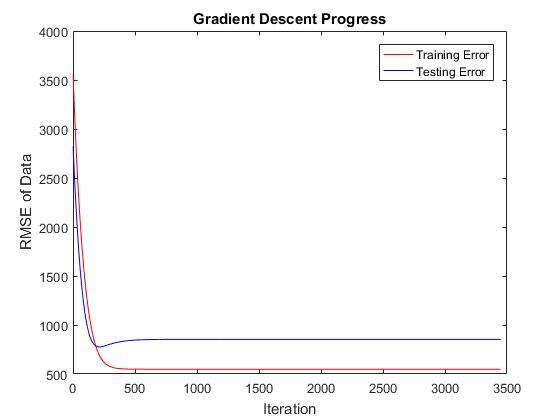
\includegraphics{part5.jpg}
\end{figure}

\end{flushleft} 

\end{document}